\newcommand{\ee}{\mathrm{e}}
\newcommand{\ii}{\mathrm{i}}
\heading{数学物理方法（上）-第5次作业}

\begin{question}
计算下列积分

1. \(\displaystyle \oint_{C} \frac{1}{z^2-1} \sin \frac{\pi z}{4} \dd{z}\)，\(C\) 分别为：

(i) \(|z|=\dfrac12\)，\qquad (ii) \(|z-1|=1\)，\qquad (iii) 心形曲线 \(r=2(1-\sin\theta)\)，\qquad (iv) \(|z|=R,\;R\to\infty\).

2. \(\displaystyle \oint_{C} \frac{1}{z^2+1} \ee^{\ii z} \dd{z}\)，\(C\) 分别为：

(i) \(|z-\ii|=1\)，\qquad (ii) \(|z|=2\)，\qquad (iii) \(|z+\ii|+|z-\ii|=2\sqrt{2}\)，\qquad (iv) 闭合曲线 \(r=3-\sin^2\frac{\theta}{4}\).

\begin{solution}
1.
(i) \(|z|=\frac12\) 的轨迹不包含 \(\pm1\)，因此积分 \(I=0\)。

(ii) \(|z-1|=1\) 的轨迹包含 \(1\)，不包含 \(-1\)，因此积分
\[ I=2\pi\ii \left.\frac{1}{z+1}\sin\frac{\pi z}{4}\right|_{z=1}=\frac{\sqrt{2}}{2}\pi\ii \]

(iii) 心形曲线的轨迹同时包含 \(\pm1\)，因此积分
\[ I=2\pi\ii \left.\frac{1}{z-1}\sin\frac{\pi z}{4}\right|_{z=-1}+2\pi\ii \left.\frac{1}{z+1}\sin\frac{\pi z}{4}\right|_{z=1}= \sqrt{2}\pi\ii \]

(iv) 当 \(R>1\) 时，由于 \(|z|=R\) 的轨迹包含 \(\pm1\)，因此积分
\[ I=2\pi\ii \left.\frac{1}{z-1}\sin\frac{\pi z}{4}\right|_{z=-1}+2\pi\ii \left.\frac{1}{z+1}\sin\frac{\pi z}{4}\right|_{z=1}= \sqrt{2}\pi\ii \]
故当 \(R\to\infty\) 时，有 \(I=\sqrt{2}\pi\ii\)。

2.
(i) \(|z-\ii|=1\) 包含 \(\ii\)，因此积分
\[ I=2\pi\ii \left.\frac{1}{z+\ii}\ee^{\ii z}\right|_{z=\ii}= \frac{\pi}{\ee} \]

(ii) \(|z|=2\) 包含 \(\pm\ii\)，因此积分
\[ I=2\pi\ii \left.\frac{1}{z-\ii}\ee^{\ii z}\right|_{z=-\ii}+2\pi\ii \left.\frac{1}{z+\ii}\ee^{\ii z}\right|_{z=\ii}=-\pi\ee+\frac{\pi}{\ee} \]

(iii) \(|z+\ii|+|z-\ii|=2\sqrt{2}\) 为焦点在 \(\pm\ii\)，长半轴为 \(\sqrt{2}\) 的椭圆，因此其包含 \(\pm\ii\)，因此积分
\[ I=2\pi\ii \left.\frac{1}{z-\ii}\ee^{\ii z}\right|_{z=-\ii}+2\pi\ii \left.\frac{1}{z+\ii}\ee^{\ii z}\right|_{z=\ii}=-\pi\ee+\frac{\pi}{\ee} \]

(iv) 闭合曲线为 \(r=3-\dfrac{1-\cos(\theta/2)}{2}=\dfrac52+\dfrac12\cos\dfrac{\theta}{2}\)，因此闭合曲线绕 \(\pm\ii\) 两点两周，因此积分
\[ I=4\pi\ii \left.\frac{1}{z-\ii}\ee^{\ii z}\right|_{z=-\ii}+4\pi\ii \left.\frac{1}{z+\ii}\ee^{\ii z}\right|_{z=\ii}=-2\pi\ee+\frac{2\pi}{\ee} \]
\end{solution}
\end{question}

\begin{question}
计算下列积分

(1) \(\displaystyle \oint_{|z|=2} \frac{\cos z}{z} \dd{z}\)，\qquad
(2) \(\displaystyle \oint_{|z|=2} \frac{z^2-1}{z^2+1} \dd{z}\)，\qquad
(3) \(\displaystyle \oint_{|z|=2} \frac{\sin \ee^{z}}{z} \dd{z}\)，\qquad
(4) \(\displaystyle \oint_{|z|=2} \frac{\ee^{z}}{\cosh z} \dd{z}\)，\qquad
(5) \(\displaystyle \oint_{|z|=2} \frac{\sin z}{z^2} \dd{z}\)，\qquad
(6) \(\displaystyle \oint_{|z|=2} \frac{\cosh z}{\ee^{z}} \dd{z}\).

\begin{solution}
(1) 围道包含了原点，因此 \(I_1 = 2\pi\ii \left.\cos z\right|_{z=0}=2\pi\ii\).

(2) 围道包含了 \(\pm\ii\)，因此
\[ I_2 = 2\pi\ii \left.\frac{z^2-1}{z-\ii}\right|_{z=-\ii} + 2\pi\ii \left.\frac{z^2-1}{z+\ii}\right|_{z=\ii} = 0. \]

(3) 围道包含了原点，因此 \(I_3=2\pi\ii \left.\sin\ee^{z}\right|_{z=0}=2\pi\ii\sin 1\).

(4) 注意到 \(\ee^{z}/(\cosh z)\) 在 \(\mathbb{C}\setminus\{\pi\ii/2,-\pi\ii/2\}\) 上解析，因此我们由柯西定理，考察如下区域可知
\begin{center}
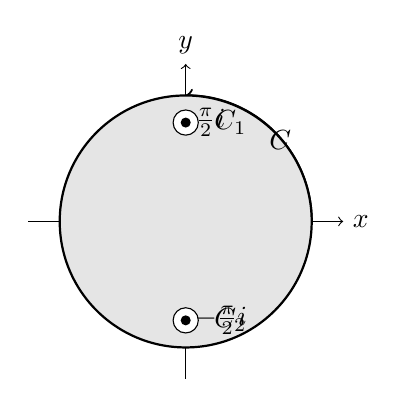
\begin{tikzpicture}[scale=0.8]
\draw[->] (-2.5,0) -- (2.5,0) node[right] {$x$};
\draw[->] (0,-2.5) -- (0,2.5) node[above] {$y$};
% Main contour C: circle of radius 2 with arrow direction
\draw[thick,->] (2,0) arc (0:90:2);
% Two small circles around singularities (fill=white for clear rendering)
\filldraw[fill=white] (0,1.57) circle (0.2);
\filldraw[fill=white] (0,-1.57) circle (0.2);
% Shading
\begin{scope}
  \fill[black!10,even odd rule] (0,0) circle (2) (0,1.57) circle (0.2) (0,-1.57) circle (0.2);
\end{scope}
% Redraw circles on top of shading
\draw[thick] (0,0) circle (2);
\filldraw[fill=white] (0,1.57) circle (0.2);
\filldraw[fill=white] (0,-1.57) circle (0.2);
\filldraw (0,1.57) circle (2pt) node[right] {$\frac{\pi}{2}i$};
\filldraw (0,-1.57) circle (2pt) node[right] {$-\frac{\pi}{2}i$};
\node at (1.5,1.3) {$C$};
\node at (0.3,1.57) [right] {$C_1$};
\node at (0.3,-1.57) [right] {$C_2$};
\end{tikzpicture}
\end{center}
\[ I_4 = \oint_{C_1} \frac{\ee^{z}}{\cosh z}\dd{z} + \oint_{C_2} \frac{\ee^{z}}{\cosh z}\dd{z}. \]
我们设 \(C_1,C_2\) 的圆半径为 \(\epsilon\)，并让 \(\epsilon\to0\)。此时在 \(C_1\) 上有，\(\cosh z \approx \ii(z-\pi\ii/2)\)，在 \(C_2\) 上有 \(\cosh z = -\ii(z+\pi\ii/2)\)，因此有
\[ I_4=2\pi\ii \left.\frac{\ee^{z}}{\ii}\right|_{z=\pi\ii/2} + 2\pi\ii \left.\frac{\ee^{z}}{(-\ii)}\right|_{z=-\pi\ii/2} = 4\pi\ii. \]

(5) 围道包含了原点，而在原点附近，\((\sin z)/z \approx 1\)，因此有 \(I_5=2\pi\ii\).

(6) \((\cosh z)/\ee^{z}\) 在 \(\mathbb{C}\) 上解析，因此 \(I_6=0\).
\end{solution}
\end{question}


\begin{question}
计算积分 \(\displaystyle \oint_{|z|=\rho} \frac{|dz|}{|z-a|^2}\) 其中 \(a\) 为任意复常数且 \(|a|\neq\rho\)，实常数 \(\rho>0\)。
\begin{solution}
做换元 \(z=\rho\ee^{\ii(\theta+\arg a)}\)，其中 \(\theta\in[-\pi,\pi]\)，因此积分变为
\[
I=\int_{-\pi}^{\pi}\frac{\rho\dd{}\theta}{\rho^2+|a|^2-2\rho|a|\cos\theta}.
\]
做换元 \(u=\tan\dfrac{\theta}{2}\)，可以得到
\[
d\theta=\frac{2\dd{u}}{1+u^2},\qquad \cos\theta=\frac{1-u^2}{1+u^2},
\]
所以有
\[
\begin{aligned}
I&=\int_{-\infty}^{\infty}\frac{2\rho\dd{u}}{(\rho^2+|a|^2)(1+u^2)-2\rho|a|(1-u^2)}\\
&=2\rho\int_{-\infty}^{\infty}\frac{du}{(\rho-|a|)^2+(\rho+|a|)^2u^2}\\
&=\frac{2\rho}{\rho^2-|a|^2}\Bigl.\arctan\Bigl(\frac{\rho-|a|}{\rho+|a|}u\Bigr)\Bigr|_{-\infty}^{\infty}.
\end{aligned}
\]

当 \(\rho<|a|\) 时，\(I=\dfrac{2\pi\rho}{|a|^2-\rho^2}\)；
当 \(\rho>|a|\) 时，\(I=\dfrac{2\pi\rho}{\rho^2-|a|^2}\)。
综上
\[
I=\frac{2\pi\rho}{|\,\rho^2-|a|^2\,|}.
\]
\end{solution}
\end{question}
